% Options for packages loaded elsewhere
\PassOptionsToPackage{unicode}{hyperref}
\PassOptionsToPackage{hyphens}{url}
\PassOptionsToPackage{dvipsnames,svgnames,x11names}{xcolor}
%
\documentclass[
  letterpaper,
  DIV=11,
  numbers=noendperiod,
  twocolumn]{scrartcl}

\usepackage{amsmath,amssymb}
\usepackage{iftex}
\ifPDFTeX
  \usepackage[T1]{fontenc}
  \usepackage[utf8]{inputenc}
  \usepackage{textcomp} % provide euro and other symbols
\else % if luatex or xetex
  \usepackage{unicode-math}
  \defaultfontfeatures{Scale=MatchLowercase}
  \defaultfontfeatures[\rmfamily]{Ligatures=TeX,Scale=1}
\fi
\usepackage{lmodern}
\ifPDFTeX\else  
    % xetex/luatex font selection
\fi
% Use upquote if available, for straight quotes in verbatim environments
\IfFileExists{upquote.sty}{\usepackage{upquote}}{}
\IfFileExists{microtype.sty}{% use microtype if available
  \usepackage[]{microtype}
  \UseMicrotypeSet[protrusion]{basicmath} % disable protrusion for tt fonts
}{}
\makeatletter
\@ifundefined{KOMAClassName}{% if non-KOMA class
  \IfFileExists{parskip.sty}{%
    \usepackage{parskip}
  }{% else
    \setlength{\parindent}{0pt}
    \setlength{\parskip}{6pt plus 2pt minus 1pt}}
}{% if KOMA class
  \KOMAoptions{parskip=half}}
\makeatother
\usepackage{xcolor}
\usepackage[top=20mm,left=20mm,right=20mm,heightrounded]{geometry}
\setlength{\emergencystretch}{3em} % prevent overfull lines
\setcounter{secnumdepth}{-\maxdimen} % remove section numbering
% Make \paragraph and \subparagraph free-standing
\ifx\paragraph\undefined\else
  \let\oldparagraph\paragraph
  \renewcommand{\paragraph}[1]{\oldparagraph{#1}\mbox{}}
\fi
\ifx\subparagraph\undefined\else
  \let\oldsubparagraph\subparagraph
  \renewcommand{\subparagraph}[1]{\oldsubparagraph{#1}\mbox{}}
\fi


\providecommand{\tightlist}{%
  \setlength{\itemsep}{0pt}\setlength{\parskip}{0pt}}\usepackage{longtable,booktabs,array}
\usepackage{calc} % for calculating minipage widths
% Correct order of tables after \paragraph or \subparagraph
\usepackage{etoolbox}
\makeatletter
\patchcmd\longtable{\par}{\if@noskipsec\mbox{}\fi\par}{}{}
\makeatother
% Allow footnotes in longtable head/foot
\IfFileExists{footnotehyper.sty}{\usepackage{footnotehyper}}{\usepackage{footnote}}
\makesavenoteenv{longtable}
\usepackage{graphicx}
\makeatletter
\def\maxwidth{\ifdim\Gin@nat@width>\linewidth\linewidth\else\Gin@nat@width\fi}
\def\maxheight{\ifdim\Gin@nat@height>\textheight\textheight\else\Gin@nat@height\fi}
\makeatother
% Scale images if necessary, so that they will not overflow the page
% margins by default, and it is still possible to overwrite the defaults
% using explicit options in \includegraphics[width, height, ...]{}
\setkeys{Gin}{width=\maxwidth,height=\maxheight,keepaspectratio}
% Set default figure placement to htbp
\makeatletter
\def\fps@figure{htbp}
\makeatother

\usepackage{amsmath}
\KOMAoption{captions}{tablesignature}
\makeatletter
\makeatother
\makeatletter
\makeatother
\makeatletter
\@ifpackageloaded{caption}{}{\usepackage{caption}}
\AtBeginDocument{%
\ifdefined\contentsname
  \renewcommand*\contentsname{Table of contents}
\else
  \newcommand\contentsname{Table of contents}
\fi
\ifdefined\listfigurename
  \renewcommand*\listfigurename{List of Figures}
\else
  \newcommand\listfigurename{List of Figures}
\fi
\ifdefined\listtablename
  \renewcommand*\listtablename{List of Tables}
\else
  \newcommand\listtablename{List of Tables}
\fi
\ifdefined\figurename
  \renewcommand*\figurename{Figura}
\else
  \newcommand\figurename{Figura}
\fi
\ifdefined\tablename
  \renewcommand*\tablename{Tabla}
\else
  \newcommand\tablename{Tabla}
\fi
}
\@ifpackageloaded{float}{}{\usepackage{float}}
\floatstyle{ruled}
\@ifundefined{c@chapter}{\newfloat{codelisting}{h}{lop}}{\newfloat{codelisting}{h}{lop}[chapter]}
\floatname{codelisting}{Listing}
\newcommand*\listoflistings{\listof{codelisting}{List of Listings}}
\makeatother
\makeatletter
\@ifpackageloaded{caption}{}{\usepackage{caption}}
\@ifpackageloaded{subcaption}{}{\usepackage{subcaption}}
\makeatother
\makeatletter
\@ifpackageloaded{tcolorbox}{}{\usepackage[skins,breakable]{tcolorbox}}
\makeatother
\makeatletter
\@ifundefined{shadecolor}{\definecolor{shadecolor}{rgb}{.97, .97, .97}}
\makeatother
\makeatletter
\makeatother
\makeatletter
\makeatother
\ifLuaTeX
  \usepackage{selnolig}  % disable illegal ligatures
\fi
\IfFileExists{bookmark.sty}{\usepackage{bookmark}}{\usepackage{hyperref}}
\IfFileExists{xurl.sty}{\usepackage{xurl}}{} % add URL line breaks if available
\urlstyle{same} % disable monospaced font for URLs
\hypersetup{
  pdftitle={Tarea 2},
  pdfauthor={Sebastián Celaya; Camila Echeverría; Francisca Vilca},
  colorlinks=true,
  linkcolor={blue},
  filecolor={Maroon},
  citecolor={Blue},
  urlcolor={Blue},
  pdfcreator={LaTeX via pandoc}}

\title{Tarea 2}
\usepackage{etoolbox}
\makeatletter
\providecommand{\subtitle}[1]{% add subtitle to \maketitle
  \apptocmd{\@title}{\par {\large #1 \par}}{}{}
}
\makeatother
\subtitle{EYP3907 - Series de Tiempo}
\author{Sebastián Celaya \and Camila Echeverría \and Francisca Vilca}
\date{}

\begin{document}
\maketitle
\ifdefined\Shaded\renewenvironment{Shaded}{\begin{tcolorbox}[enhanced, breakable, borderline west={3pt}{0pt}{shadecolor}, interior hidden, frame hidden, boxrule=0pt, sharp corners]}{\end{tcolorbox}}\fi

\hypertarget{introducciuxf3n}{%
\subsection{Introducción}\label{introducciuxf3n}}

Utilizando una base de datos que contiene información sobre el ancho de
los anillos de árboles pertenecientes a la especie \emph{Pino
Silvestre}, que puede encontrarse en el siguiente
\href{https://www.ncei.noaa.gov/pub/data/paleo/treering/measurements/europe/norw001x-rwl-noaa.txt}{link},
ajustaremos un modelo ARMA y realizaremos diversos procedimientos para
comprobar su ajuste.

\hypertarget{anuxe1lisis-exploratorio}{%
\subsection{Análisis exploratorio}\label{anuxe1lisis-exploratorio}}

La fig-exp1 muestra los valores del ancho del anillo registrados entre
los años 1721 y 1889.

\begin{figure}[H]

{\centering 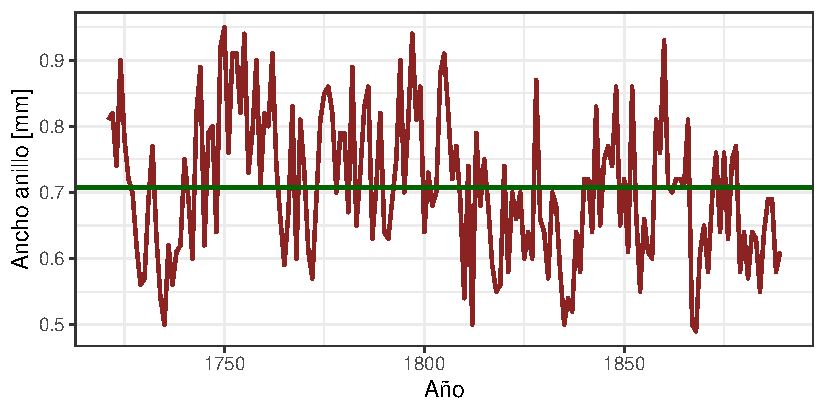
\includegraphics{CopyOfpdf_tarea2_files/figure-pdf/fig-exp1-1.pdf}

}

\caption{\label{fig-exp1}Variación del ancho del anillo}

\end{figure}

Gracias a la fig-exp2, es posible ver que la mediana de estos datos se
encuentra cercana a 0.7 y que no tenemos datos atípicos, aunque la
segunda mitad de las observaciones parecieran estar ligeramente más
dispersa que la primera.

\begin{figure}[H]

{\centering 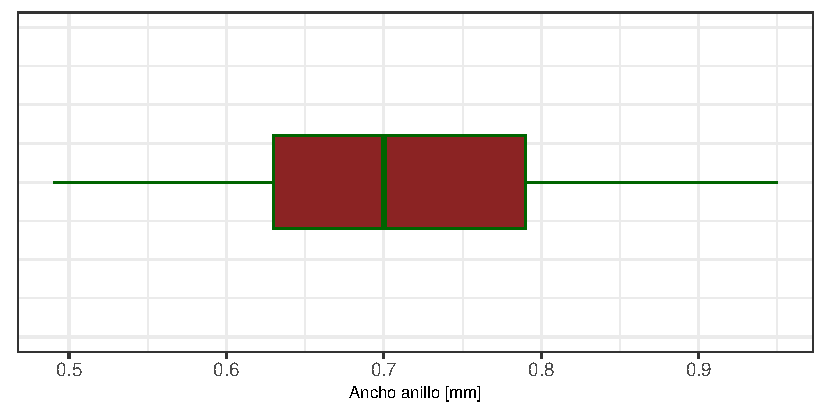
\includegraphics{CopyOfpdf_tarea2_files/figure-pdf/fig-exp2-1.pdf}

}

\caption{\label{fig-exp2}Boxplot de ancho de anillo}

\end{figure}

\begin{figure}[H]

{\centering 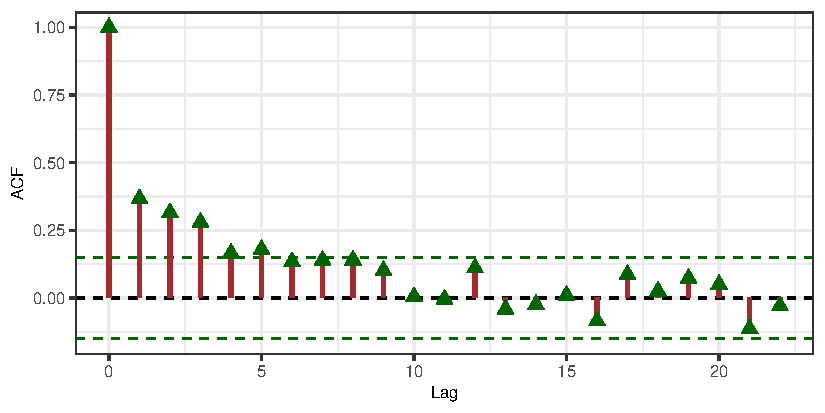
\includegraphics{CopyOfpdf_tarea2_files/figure-pdf/fig-exp3-1.pdf}

}

\caption{\label{fig-exp3}Gráfico de Autocorrelación}

\end{figure}

\begin{figure}[H]

{\centering 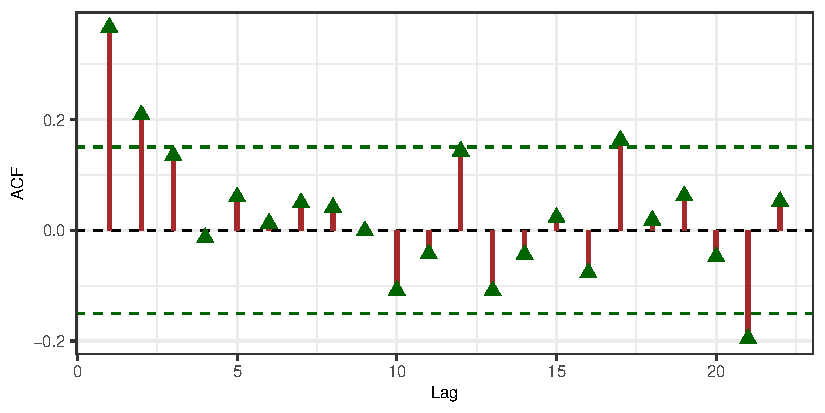
\includegraphics{CopyOfpdf_tarea2_files/figure-pdf/fig-exp4-1.pdf}

}

\caption{\label{fig-exp4}Gráfico de Autocorrelación Parcial}

\end{figure}

Luego, en los gráficos de la fig-exp3 y la fig-exp4 podemos ver la
estructura de correlación de los datos. Si bien no se puede detectar
estacionalidad a simple vista, las observaciones sí presentan altos
niveles de correlación.

\hypertarget{ajuste-de-un-modelo-arma}{%
\subsection{Ajuste de un modelo ARMA}\label{ajuste-de-un-modelo-arma}}

A simple vista, de los gráficos de ACF y PACF, vemos que nuestro modelo
tiene estructura de un ARMA. Sin embargo, al usar la función
\texttt{auto.arima()} como guía se recomienda usar un modelo MA(1), pero
al hacerle las pruebas a los residuos, este rechaza el test de blancura.
Por lo que, nuestra propuesta es un modelo arma(1,1), para que este sea
capaz de capturar toda la estructura de la serie temporal.

\hypertarget{a-significancia-estaduxedstica-de-los-coeficientes-del-modelo}{%
\subsubsection{a) Significancia estadística de los coeficientes del
modelo}\label{a-significancia-estaduxedstica-de-los-coeficientes-del-modelo}}

Sabemos que los coeficientes del modelo deben cumplir con ser
estadísticamente significantes, por lo que al revisar el valor-p
asociado a cada coeficiente del modelo, es claro notar que todos son
significativos, tal como se muestra en la tabla 1:

\hypertarget{b-estacionaridad-e-invertibilidad-del-modelo-arma}{%
\subsubsection{b) Estacionaridad e invertibilidad del modelo
ARMA}\label{b-estacionaridad-e-invertibilidad-del-modelo-arma}}

Una forma sencilla de comprobar la estacionalidad en los datos es con el
test de Dickey-Fuller, el cual nos da un valor-p de 0.01 que al ser
menor al \(5\%\) de significancia se rechaza la hipótesis nula de que
los datos son estacionales. Por otro lado, una forma sencilla de
verificar invertibilidad del modelo ARMA(1,1), es de forma gráfica,
comprobando que los coeficientes se encuentren al interior de la
circunferencia unitaria, lo que puede ser apreciado en la fig-exp5 :

\begin{verbatim}
null device 
          1 
\end{verbatim}

\hypertarget{c-test-de-blancura---homocedasticidad-y-normalidad-de-los-residuos}{%
\subsubsection{c) Test de blancura - homocedasticidad y normalidad de
los
residuos}\label{c-test-de-blancura---homocedasticidad-y-normalidad-de-los-residuos}}

Sabemos que los residuos del modelo, es decir, lo que no es capaz de
explicar el modelo ARMA(1,1), debe cumplir con ser normales, tener
varianza constante e idealmente provenir de un ruido blanco. Para ello
veremos diferentes test que se le pueden aplicar para comprobar ello:

\begin{itemize}
\tightlist
\item
  Usando el estadístico de Ljung-Box es
\end{itemize}

\begin{figure}[H]

{\centering 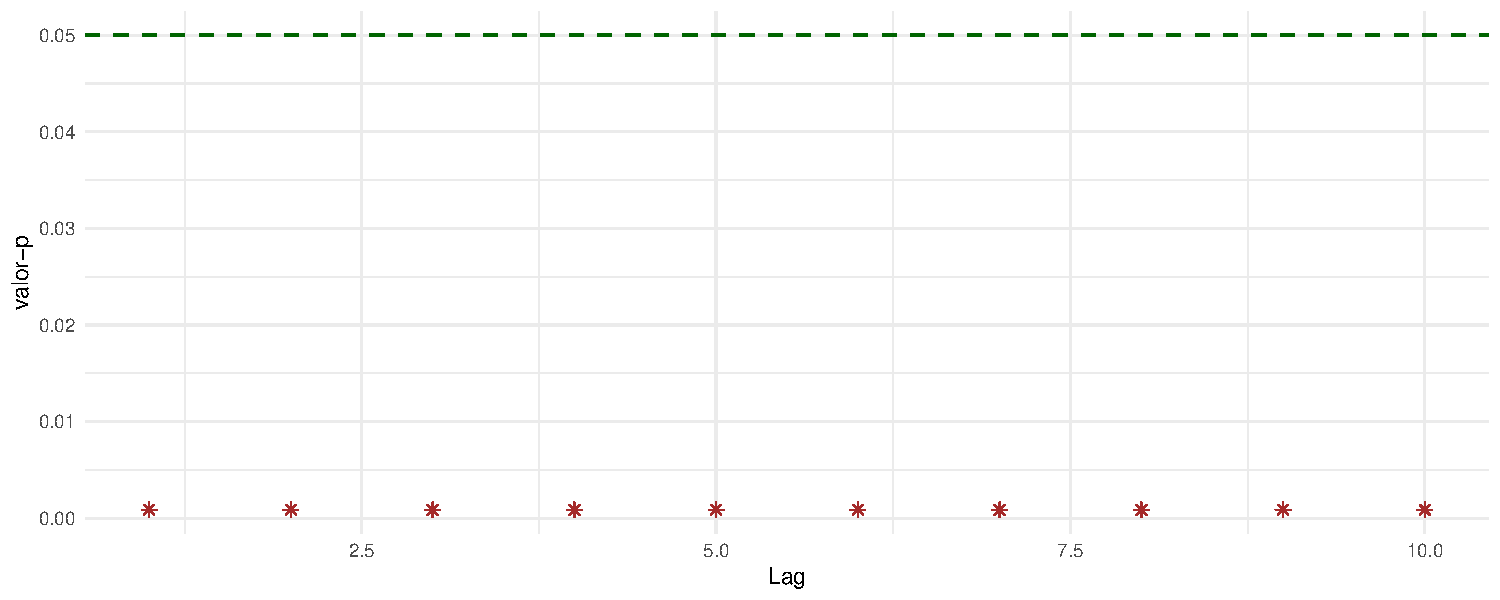
\includegraphics{CopyOfpdf_tarea2_files/figure-pdf/unnamed-chunk-10-1.pdf}

}

\end{figure}

\hypertarget{d-es-necesario-realizar-una-transformaciuxf3n-de-box-cox}{%
\subsubsection{d) ¿Es necesario realizar una transformación de
Box-Cox?}\label{d-es-necesario-realizar-una-transformaciuxf3n-de-box-cox}}

\begin{verbatim}
Time Series:
Start = 170 
End = 170 
Frequency = 1 
[1] 0.7087664
\end{verbatim}

\begin{verbatim}
Time Series:
Start = 170 
End = 170 
Frequency = 1 
          80%       95%
170 0.5516832 0.4685284
\end{verbatim}

\begin{verbatim}
Time Series:
Start = 170 
End = 170 
Frequency = 1 
          80%       95%
170 0.8658497 0.9490045
\end{verbatim}

\hypertarget{muxe9todo-de-whittle}{%
\subsection{Método de Whittle}\label{muxe9todo-de-whittle}}

Ahora si se ajustan los datos con el método de Whittle, también con un
modelo ARMA(1,1), obtenemos coeficientes significativos. Además, si
usamos la función \texttt{forecast()} obtenemos que la predicción de la
dimensión del anillo para el siguiente año es de 0.661 y construyendo un
intervalo de confianza al \(95\%\) es de {[}0.605,0.716{]}. Los cuales
al compararlos con los obtenidos con el método de Durvin-Levinson vemos
que las diferencias son mínimas.

Una forma sencilla de comparar los ajustes es mediantes un gráfico de
líneas para visualizar que tanto logran extraer la información de los
datos originales como en la fig 6

\begin{figure}[H]

{\centering 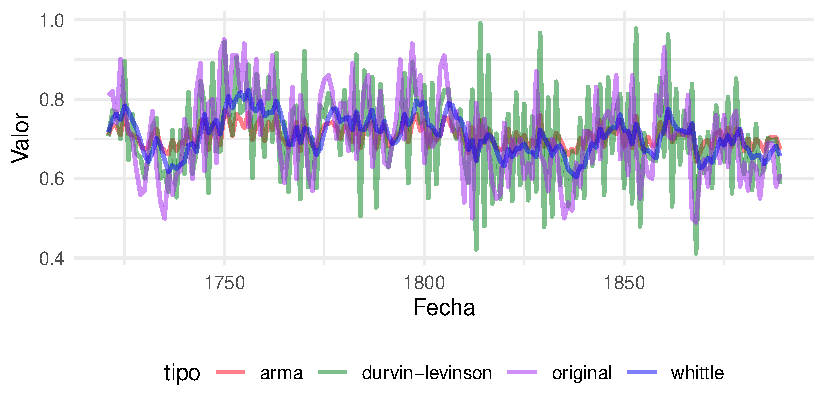
\includegraphics{CopyOfpdf_tarea2_files/figure-pdf/fig-exp6-1.pdf}

}

\caption{\label{fig-exp6}Compara}

\end{figure}

De la fig exp6, vemos claramente que el ajuste mediante el algortimo de
Durvin-Levinson y por el de Whittle, son bastantes similares, por lo
mismo sus predicciones tambien lo son. Por otro lado, vemos como el
modelo arma no logra capturar por completo la variabilidad de los datos
como si lo hacen los otros métodos.

\hypertarget{comparaciuxf3n-de-ajustes}{%
\subsection{Comparación de ajustes}\label{comparaciuxf3n-de-ajustes}}

Finalmente, una forma bastante sencilla de comparar los modelos es
mediante medidas para evaluar el error las cuales se presentan en la
tabla n+1

\begin{table}[H]
\centering
\begin{tabular}{| c | c | c | c | c | c | c | c |}
\hline
 & ME & RMSE & MAE & MPE & MAPE & MASE \\
\hline
ARMA(1,1) & 0.15 & 0.12 & 16.35\\
\hline
Durvin- \n Levinson & 0.23 & 0.14 & 17.00 \\
\hline
Whittle & 0.23 & 0.14 & 17.00 \\
\bottomrule
\end{tabular}
\caption{Medidas de calidad de ajuste}

\end{table}



\end{document}
